\documentclass{article}
\usepackage{icomp2026_conference,times}

\usepackage[T1]{fontenc}
\usepackage[utf8]{inputenc}
\usepackage[english]{babel}
\usepackage{hyperref}
\usepackage{url}
\usepackage{booktabs}
\usepackage{nicefrac}
\usepackage{microtype}
\usepackage{xcolor}
\usepackage{graphicx}
\usepackage{subcaption}
\usepackage{amsmath,amssymb,amsfonts}
\usepackage{amsthm}
\usepackage{float}

\newtheorem{proposition}{Proposition}
\newtheorem{criterion}{Criterion}

\usepackage[capitalize]{cleveref}
\crefname{section}{section}{sections}
\Crefname{section}{Section}{Sections}
\crefname{table}{table}{tables}
\Crefname{table}{Table}{Tables}

\title{Delay-Embedding Analysis of Neural Network Training Logs:\\
Preconditions, Negative Results, and Validated Driver Recovery}

\author{
  Nickolay Karlov\\
  MIPT\\
  Moscow, Russia\\
  \texttt{karlov.na@phystech.edu}\\
  \And
  Alexey Kravatskiy\\
  MIRIAI\\
  Moscow, Russia\\
  \texttt{kravatskii.a@miriai.org}\\
}

\icomparxivcopy   % named preprint: show the authors, without claiming publication

\begin{document}

\maketitle

\begin{abstract}
Empirical dynamic modelling promises to recover the structure of a high-dimensional
system from scalar observations, which makes it attractive for monitoring neural network
training from logs that consume negligible memory. This report establishes when that
promise is redeemable. The embedding theorems of Takens and Stark reconstruct a compact
invariant set that the trajectory revisits; we measure recurrence directly and find that
raw training logs do not satisfy this precondition, with recurrence rates falling to zero
under temporal exclusion while a reference chaotic attractor retains $0.93$. We then
report three candidate signals for the delayed generalisation phenomenon known as
grokking, each of which separates training runs convincingly and none of which survives a
controlled comparison: an intrinsic-dimension estimate that reproduces closed-form
constants of a straight line, a function-space velocity that tracks weight decay rather
than generalisation, and a shared-manifold coupling that tracks configuration rather than
the transition. Against these we set a positive result obtained in the regime where
Stark's theorem does apply. Convergent cross mapping recovers an externally injected
driver from a single one-dimensional loss log in seven of eight coupled runs across two
architectures, with no false positives in five control runs whose driver is logged but
never applied, and with a limitation for strictly periodic drivers that we characterise
quantitatively. Finally, a factorial study of thirty runs shows that the delay reported in
earlier work lies far outside the distribution produced by its own configuration. We
conclude with a control protocol that would have falsified each negative result before
publication.
\end{abstract}

\textbf{Keywords:} empirical dynamic modelling, delay embedding, surrogate data,
convergent cross mapping, grokking, training diagnostics.

\section{Introduction}\label{sec:intro}

A training run exposes very little of itself cheaply. Weights and activations are large
and expensive to store, whereas scalar logs such as the training loss, the validation
loss and the parameter norm cost almost nothing. If the geometry of the underlying
optimisation could be reconstructed from those scalars, monitoring would become
inexpensive and architecture independent. This is the premise of empirical dynamic
modelling, and it rests on the embedding theorems of Takens \citep{takens1981detecting}
and, for forced systems, of Stark \citep{stark1999delay, stark2003delay}.

Earlier work in this project applied that premise to grokking, the delayed generalisation
reported by \citet{power2022grokking}, and proposed that a collapse in the intrinsic
dimension of a delay-embedded weight-norm series precedes the transition. The present
report re-examines that proposal, reports what replaces it, and states the boundary that
separates the two.

The organising claim is the following. The embedding theorems reconstruct a compact
invariant set that the trajectory revisits. A training run driven by an external signal
with its own attractor satisfies this requirement by construction. The intrinsic
optimisation transient does not. Results that respect this boundary reproduce across
architectures and controls; results that cross it recover artefacts of trajectory
smoothness or of run configuration. \Cref{sec:preconditions} measures the precondition,
\cref{sec:negative} reports three signals that violate it, \cref{sec:ccm} reports the
positive result obtained inside it, and \cref{sec:phenomenon} re-examines the phenomenon
itself. \Cref{sec:protocol} states the protocol we recommend.

\section{Preconditions for delay embedding}\label{sec:preconditions}

Takens' theorem and its extensions guarantee that a delay map is an embedding of an
\emph{invariant set}. The guarantee is asymptotic and geometric: the orbit must return
near its past states, so that neighbours in the reconstructed space are dynamically
related rather than merely adjacent in time. When this fails, nearest-neighbour
statistics measure the local tangent to the trajectory instead of the geometry of an
attractor, a distortion first identified by \citet{theiler1986spurious}.

We therefore measure recurrence before invoking any theorem. For a delay-embedded series
we fix a neighbourhood radius once, as a low quantile of all pairwise distances, and
report the recurrence rate as a function of a temporal exclusion window. Fixing the radius
once is essential; recomputing it after each exclusion would force the recurrence rate to
equal the quantile for any input whatsoever, an error we made and corrected during this
work. The shape of the resulting profile separates the two cases of interest. On an
invariant set the rate falls to a positive plateau, because genuine returns occur at all
temporal separations beyond the orbit's period. On a transient the rate decays towards
zero, because every close pair was adjacent in time.

The estimator is calibrated on systems with known answers. A Lorenz-63 trajectory retains
$0.93$ of its recurrence rate at the widest exclusion, whereas a monotone ramp, which has
no dynamics at all, decays to exactly $0.00$. \Cref{fig:preconditions} applies it to the
training logs.

\begin{figure}[H]
\centering
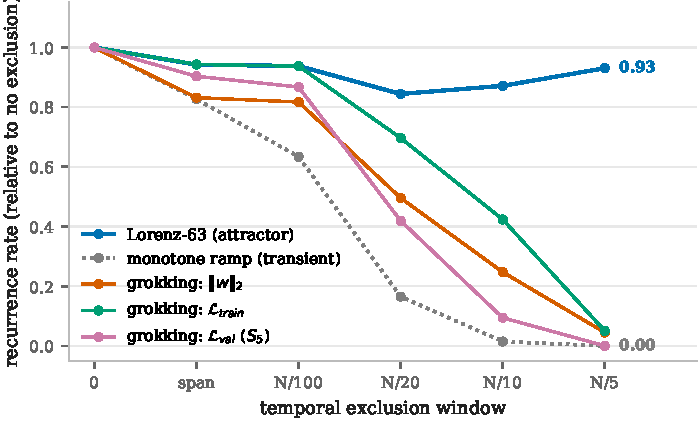
\includegraphics[width=0.72\textwidth]{figures/fig1_preconditions.pdf}
\caption{Recurrence rate as a function of the temporal exclusion window, normalised by the
rate at zero exclusion. The Lorenz attractor holds a plateau, while all three training
observables decay towards the monotone-ramp reference. The training trajectories do not
revisit their past states, so no invariant set is available for the embedding theorems to
reconstruct.}
\label{fig:preconditions}
\end{figure}

All three training observables behave like the transient reference rather than like the
attractor. The validation loss of the $S_5$ runs reaches a ratio of $0.000$ and the
weight norm falls between $0.00$ and $0.07$. This is a structural fact about optimisation
rather than a defect of any particular estimator, and it explains why dimension estimates
computed on these logs are not measurements of an attractor.

One caveat constrains the use of this diagnostic. Independent noise also produces close
pairs at arbitrary temporal separations and therefore also scores near unity. Recurrence
separates smooth transients from everything else; it does not separate an attractor from
noise, and a determinism test must follow it. We return to this point in
\cref{sec:negative}.

\section{Signals that do not survive controlled comparison}\label{sec:negative}

\subsection{Intrinsic dimension of the weight-norm trajectory}

The Levina--Bickel maximum likelihood estimator \citep{levina2004maximum} applied to a
sliding window of the weight-norm series produces a curve that rises during memorisation
and falls before generalisation. Three observations remove its interpretation as a
dimension.

First, the reported values are closed-form constants of a straight line. For a locally
straight and uniformly sampled trajectory the $k$ nearest neighbours lie at temporal
offsets $1,\dots,k$, so the estimate depends only on $k$ and on the exclusion window and
not on the data. At $k=5$ that constant is $1.33$ without exclusion and $10.76$ with an
exclusion of fourteen samples. The published control runs report $1.33$ to $1.40$ and
$8.84$ to $12.93$ respectively, and a synthetic straight line reproduces both plateaus to
two decimal places.

Second, the estimate is not identifiable. Doubling the embedding dimension approximately
doubles the reported value on these logs, whereas a genuine low-dimensional attractor
leaves it unchanged. Even a Lorenz trajectory is unresolvable at the window lengths used,
which places the requirement on the data rather than on the estimator.

Third, the windows were labelled by their centres, so each estimate incorporated data from
after the step it was assigned to. Under causal labelling the reported lead over the
transition does not survive.

Averaging the per-point estimates also inflates them relative to pooling the likelihood,
as \citet{mackay2005comments} note; the correction changes the level but not the
conclusion, because the underlying quantity is not identifiable in the first place.

\subsection{Function-space velocity}

The preceding failure suggests an observable that cannot be a smoothness artefact of the
weight norm. We therefore recorded, at each logged step, the logits of a fixed probe set
of training inputs, centred each example's logit vector over classes and normalised it to
unit length. The resulting series is invariant to the uniform rescaling of logits that
weight decay induces, so a change in it indicates that the computed function has moved
rather than that its confidence scale has changed. The median per-example movement of the
normalised logits separates a grokking run from a run without weight decay by a factor of
approximately $360$.

The separation does not survive its control. We trained runs in which weight decay is
held at $1.0$ and only the quantity of training data is reduced, so that the model
memorises and never generalises. These runs exhibit \emph{higher} sustained velocity
($7.26\times10^{-2}$ and $5.30\times10^{-2}$) than the run that groks
($1.84\times10^{-2}$), while the only run far below all others is the one without weight
decay ($1.53\times10^{-4}$). Every run with weight decay lies within a factor of five of
every other. The statistic therefore measures the reorganisation that regularisation
imposes on the function, and among regularised runs it is, if anything, inversely related
to generalisation.

\subsection{Shared-manifold coupling}

Both preceding failures are statistics of a single transient series. Cross mapping asks a
different question, namely whether two observables lie on a common manifold, and that
question is well posed on a transient because it requires no recurrence of either series
alone. We therefore tested whether the training loss and the parameter norm, both
available without any validation data, share a manifold, and whether the coupling changes
at the transition.

The result appeared decisive. \Cref{fig:confound}(a) shows a clean separation with no
overlap: the three runs with a delayed transition have median coupling between $1.00$ and
$1.15$, while the four runs without lie between $2.87$ and $5.61$.

\begin{figure}[H]
\centering
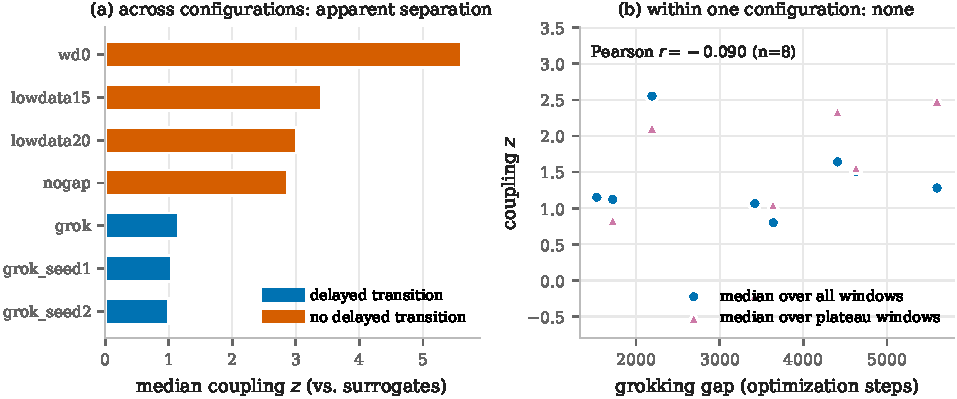
\includegraphics[width=0.92\textwidth]{figures/fig4_confound_free.pdf}
\caption{(a) Median coupling between the training loss and the parameter norm separates
runs with a delayed transition from runs without. (b) The same statistic across eight runs
of a single configuration, in which only the split and initialisation seeds vary. The gap
spans $1290$ to $5600$ steps and the coupling is unrelated to it. The separation in panel
(a) reflects configuration, not the transition.}
\label{fig:confound}
\end{figure}

Two checks dissolve it. Within individual runs the statistic does not move at the moment
of generalisation; the apparent step in an aggregate over runs arises from averaging runs
whose transitions occur at different steps. More importantly, the grouping in panel (a)
coincides exactly with configuration, since the low group consists of the runs with a
training fraction of $0.3$ and weight decay of $1.0$ and the high group contains every
other setting. We therefore held configuration fixed and varied only the split and
initialisation seeds, which the study of \cref{sec:phenomenon} shows produce gaps between
$1290$ and $5600$ steps. The expected sign was recorded before the runs were executed.
The observed correlation between the gap and the coupling is $-0.090$ (Pearson) and
$+0.214$ (Spearman) over eight runs, that is, nothing, and for plateau windows it is
weakly positive, which is the opposite of the prediction. Within one configuration the
coupling spans $0.80$ to $2.55$, against $1.0$ to $5.6$ across configurations.

\subsection{A common failure mode}

The three signals fail in the same way. Each separates \emph{configurations} rather than
\emph{transitions}, and each is confirmed by a comparison in which the runs differ in more
than the property of interest. The controls that falsify them share every feature with the
positive runs except the mechanism under test: weight decay held fixed while data is
varied, or configuration held fixed while seeds are varied. We regard this, rather than
any individual negative result, as the principal methodological lesson.

\section{Driver recovery in the regime where the theorems apply}\label{sec:ccm}

Stark's extension of Takens' theorem covers a system driven by an external signal that
possesses its own attractor \citep{stark1999delay, stark2003delay}. A training run
modulated by an injected driver satisfies that hypothesis by construction, which makes it
the natural setting in which to ask whether anything at all is recoverable from a
one-dimensional log.

\subsection{Design}

We use two independent settings. The first consists of existing logs from a ResNet-18
trained on CIFAR-10, in which a fraction of each batch's labels is corrupted according to
a driver logged alongside the loss. The second reproduces the design in this work, using a
one-layer transformer on modular addition with drivers under our control. In both cases
the ground truth is known, and in both cases the essential control is a \emph{ghost}
driver, which is logged exactly like a real one while the batch is returned unmodified.
A ghost run shares the architecture, the schedule, the loss trajectory and the logging
cadence of a coupled run and differs only in whether coupling exists.

Detection uses convergent cross mapping \citep{sugihara2012detecting}: the response is
delay embedded and used to predict the driver, on the reasoning that if the driver forces
the response then the reconstructed manifold of the response carries information about the
driver's state. Significance is assessed against two nulls. The first uses iterative
amplitude-adjusted Fourier surrogates \citep{theiler1992testing, schreiber1996improved},
which preserve the power spectrum and the exact value distribution of the driver while
destroying its alignment with the response. The second rotates the driver in time, which
preserves every value and changes only the alignment. No result is reported without them.

\subsection{Results}

\begin{figure}[H]
\centering
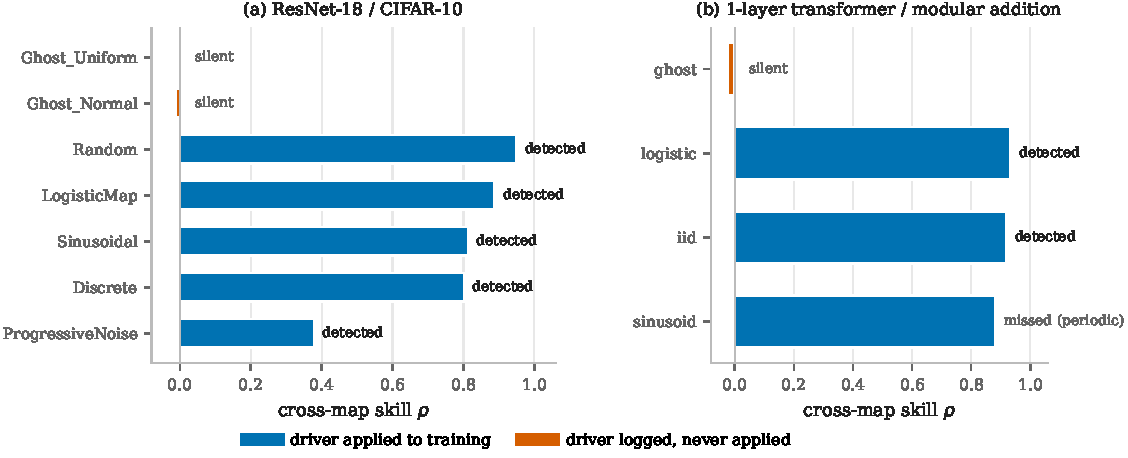
\includegraphics[width=0.95\textwidth]{figures/fig2_driver_recovery.pdf}
\caption{Cross-map skill for every run in both settings. Drivers that were applied to
training are recovered from the loss log alone; drivers that were logged but never applied
are not. The single missed detection is the smooth periodic driver discussed in
\cref{sec:periodic}.}
\label{fig:recovery}
\end{figure}

\Cref{fig:recovery} summarises both settings. In the ResNet setting all five coupled
drivers are detected, with skills between $0.379$ and $0.949$ and $p \le 0.05$ under both
nulls, and all ghost runs remain silent at skills of $-0.011$ and $-0.007$. In the
transformer setting the chaotic and independent drivers are detected at $0.934$ and
$0.919$ and the ghost remains silent at $-0.024$. Across both settings, seven of eight
coupled runs are detected and none of the five ghost runs produces a false positive.

The ghost runs carry the argument. They share the training trend with the coupled runs, so
their near-zero skill excludes the explanation that defeated the signals of
\cref{sec:negative}, namely that a statistic separates runs because their loss curves have
different shapes.

\begin{figure}[H]
\centering
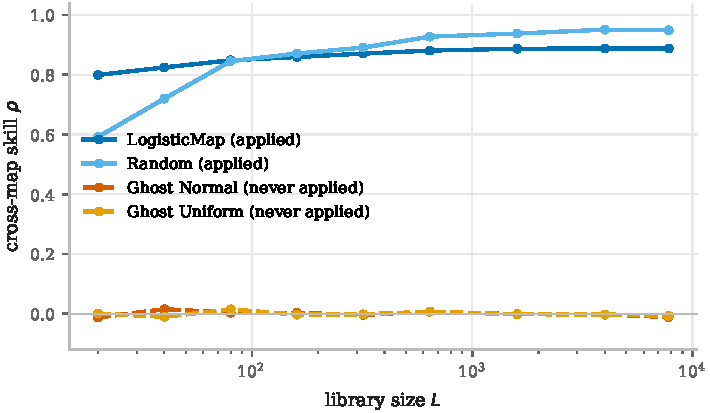
\includegraphics[width=0.72\textwidth]{figures/fig3_convergence.pdf}
\caption{Cross-map skill against library size. Coupled runs improve as the manifold is
sampled more densely, which is the convergence signature that distinguishes causation from
coincidental correlation. Ghost runs remain at zero for every library size.}
\label{fig:convergence}
\end{figure}

\Cref{fig:convergence} shows the convergence criterion that gives the method its name. The
skill of the coupled runs rises with library size, most clearly for the independent driver,
which climbs from $0.59$ to $0.95$. The ghost runs show no such rise, and no level.

One preprocessing choice deserves emphasis because it initially inverted the conclusion.
Differencing the response is the obvious way to remove the training trend, but it is a
high-pass filter and therefore removes slow drivers. The periodic drivers have the
strongest direct coupling of any run, with correlations of $0.69$ and $0.58$ against the
loss, yet they cross map at $0.09$ and $0.12$ after differencing and at $0.81$ and $0.80$
without it. The trend requires no manual removal, because both nulls and the ghost runs
already control for it.

\subsection{A limitation for periodic drivers}\label{sec:periodic}

The one missed detection is instructive and is not repaired by a better statistic. The
smooth sinusoidal driver of the transformer setting yields a cross-map skill of $0.882$,
which is high, but its surrogates reach between $0.87$ and $0.94$, which is equally high.
The reason is structural. The loss reveals the phase of the cycle, and any series of the
same period, whether a spectrum-preserving surrogate or the driver rotated in time, is a
deterministic function of that phase and is therefore equally predictable from it.
Spectrum-preserving nulls consequently have no power against a strictly periodic driver.
The corresponding driver in the ResNet setting is detected only because it is quantised to
ninety-five distinct values, so its surrogates depart from it considerably further. A
different null, for example a driver of a different period, would be required.

\subsection{The method is not discriminative between a run's own metrics}

For completeness we applied the same procedure to pairs of observables within single
uninjected runs. Eleven of sixteen directed pairs pass both nulls, with skills as high as
$1.000$. This is consistent with the theory, since the training loss, the validation loss
and the parameter norm are three observations of one system, but it means that cross
mapping between a run's own metrics carries no information about the transition and should
not be interpreted as a discovery.

\section{The delayed transition is not typical of its configuration}\label{sec:phenomenon}

The configuration used in earlier work seeds a single random stream from which the
train and validation split is drawn and from which the model initialisation then
continues. Consequently a change of seed alters which examples are used for training and
what the initial weights are, and the two cannot be distinguished. We separated them by
restarting the stream between the two steps, verified that the modification is inert when
unused and that it decouples the two factors in both directions, and then ran a factorial
study of six splits by five initialisations, with weight decay fixed throughout.

\begin{figure}[H]
\centering
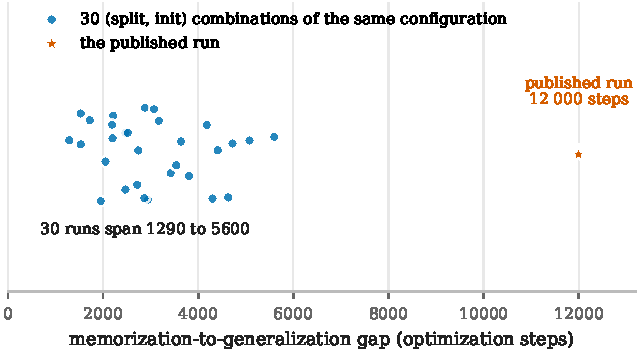
\includegraphics[width=0.72\textwidth]{figures/fig5_delay_distribution.pdf}
\caption{Memorisation-to-generalisation gap for thirty runs of one configuration, varying
only the split and initialisation seeds. Every run generalises and every gap lies between
$1290$ and $5600$ steps. The delay reported in earlier work lies far outside this
distribution.}
\label{fig:delays}
\end{figure}

All thirty runs generalise, with gaps between $1290$ and $5600$ steps, a median of $2875$
and a standard deviation of $1130$. \Cref{fig:delays} places the previously reported delay
of approximately $12\,000$ steps against that distribution. Five of the thirty runs use the
same split as the published run, so the discrepancy is not a property of the split alone.

The variance decomposition is inconclusive by design rather than by accident. The split
accounts for $19.8\%$ of the variance in the gap and the initialisation for $23.8\%$, with
the remainder in the interaction. Neither factor dominates. We note that a partial
analysis of the first fifteen cells indicated the opposite, with the split accounting for
$43\%$ against $17\%$ for the initialisation, which is a caution against reading factorial
studies before they complete.

\section{Recommended protocol}\label{sec:protocol}

The following four requirements would have falsified each negative result of
\cref{sec:negative} before it was written up, at a cost of well under an hour of
computation each.

\begin{enumerate}
\item \textbf{State and measure the precondition.} Report recurrence before invoking an
embedding theorem. If the trajectory does not revisit its past states, the language of
attractors and their dimensions does not apply, whatever number an estimator returns.

\item \textbf{Test every claim against surrogates.} A statistic that does not exceed an
amplitude-adjusted Fourier surrogate ensemble is reporting the linear autocorrelation of
the series. Where the driver is periodic, add a rotation null, and note that neither has
power in the strictly periodic case.

\item \textbf{Include a control that shares everything but the mechanism.} The ghost
drivers of \cref{sec:ccm} are the model: identical architecture, schedule, loss trajectory
and logging, differing only in whether coupling exists. Controls that differ in several
respects at once cannot discriminate, which is precisely how the signals of
\cref{sec:negative} appeared convincing.

\item \textbf{Hold configuration fixed and vary only seeds, with the expected sign
recorded in advance.} Any statistic proposed as a predictor of the transition must
correlate with the delay across runs of one configuration. This test is inexpensive and it
falsified the most promising of our candidates.
\end{enumerate}

Two further practices proved necessary in the course of this work. Estimators should be
calibrated against systems with known answers before being applied to project data, since
two of our own diagnostics were found to be circular or mis-specified in exactly that way.
Preprocessing should be justified per series rather than adopted globally, since
subtracting a moving average manufactures structure in sparse series and differencing
removes slow drivers.

\section{Conclusion}\label{sec:concl}

Delay-embedding methods are applicable to neural network training logs in a narrower
regime than the earlier proposal assumed, and within that regime they work well. When an
external driver possessing its own attractor forces training, convergent cross mapping
recovers it from a single scalar loss log, in seven of eight coupled runs across two
architectures and with no false positives among five runs whose driver was logged but
never applied. The recovered quantity is causal rather than correlational, it requires no
validation data, and it is obtained from a log that costs nothing to store.

The intrinsic optimisation transient does not admit the same treatment. It does not
revisit its past states, and the three statistics we examined that appeared to detect the
grokking transition were found instead to separate run configurations. The phenomenon
itself is also less stable than previously supposed, since thirty runs of the published
configuration produce delays between $1290$ and $5600$ steps against a reported value of
approximately $12\,000$.

We therefore recommend that future work on this problem either restricts itself to the
driven regime, where the theory applies and validation is possible, or targets the
question that the present negative results leave open, namely whether any training-side
observable distinguishes a run that will generalise from a run that will not when
configuration is held fixed. None of the observables examined here, comprising the
parameter norm, the trajectory roughness, the intrinsic dimension, the function-space
velocity and the shared-manifold coupling, is able to do so.

\bibliographystyle{icomp2026_conference}
\bibliography{references}

\end{document}
